\documentclass[a4paper,12pt,eval,firamath]{nsi}
\usepackage{ulem}
\begin{document}
\titre{Contrôle 02}
\classe{NSI2}
\maketitle


\section*{Exercice 1 \small{\hfill bases de données, langage SQL}}

L'énoncé de cet exercice utilise les mots du langage SQL suivants :\\

 \mintinline{sql}{SELECT FROM, WHERE, JOIN ON, INSERT INTO VALUES}\\
 \mintinline{sql}{UPDATE, SET, DELETE, COUNT, AND, OR}\\

Pour la gestion des réservations clients, on dispose d'une base de données nommée \mintinline{sql}{gare} dont le schéma relationnel est le suivant :\\

\texttt{\textbf{Train} (\uline{numT}, provenance, destination, horaireArrivee, horaireDepart)}\\

\texttt{\textbf{Reservation} (\uline{numR}, nomClient, prenomClient, prix, \dashuline{numT})}\\

Les attributs soulignés en trait plein sont des clés primaires. L'attribut souligné en pointillés est une clé étrangère : \mintinline{sql}{Reservation.numT} fait référence à la clé primaire \mintinline{sql}{Train.numT}.\\

Les attributs \mintinline{sql}{horaireDepart} et \mintinline{sql}{horaireArrivee} sont de type  \mintinline{sql}{TIME} et s'écrivent selon le format \mintinline{sql}{hh:mm}, où \mintinline{sql}{hh} représente les heures et \mintinline{sql}{mm} les minutes.\\

\begin{enumerate}
      \item Quel nom générique donne-t-on aux logiciels qui assurent, entre autres, la persistance des données, l'efficacité de traitement des requêtes et la sécurisation des accès pour les bases de données ?\\
      
      \carreauxseyes{16}{1.6}
      
      \item \begin{enumalph}
                  \item On considère les requêtes SQL suivantes :
                        
                        \begin{sql}
                              \begin{minted}{sql}
            DELETE FROM Train WHERE numT = 1241 ;
            DELETE FROM Reservation WHERE numT = 1241 ;
      \end{minted}
                        \end{sql}
                        
                        Sachant que le train n°1241 a été enregistré dans la table \mintinline{sql}{Train} et que des réservations pour ce train ont été enregistrées dans la table \mintinline{sql}{Reservation}, expliquer pourquoi cette suite d'instructions renvoie une erreur.\\

                        \carreauxseyes{16}{2.4}

                  \item Citer un cas pour lequel l'insertion d'un enregistrement dans la table \mintinline{sql}{Reservation} n'est pas possible.\\
                  
                  \carreauxseyes{16}{2.4}
                        
            \end{enumalph}
      \item Écrire des requêtes SQL correspondant à chacune des instructions suivantes :
            \begin{enumalph}
                  
                  \item Donner tous les numéros des trains dont la destination est « Lyon ».\\
                  
                  \carreauxseyes{16}{4}
                  
                  \item Ajouter une réservation n°1307 de 33 € pour M. Alan Turing dans le train n°654.\\
                  
                  \carreauxseyes{16}{4}


                  \item Suite à un changement, l'horaire d'arrivée du train n°7869 est programmé à 08: 11.\\
                        Mettre à jour la base de données en conséquence.\\

                        \carreauxseyes{16}{4}
                  \item Produire la table des noms et prénoms de tous les clients qui ont effectué une réservation pour un train partant de Paris et allant à Marseille.\\
                  
                  \carreauxseyes{16}{4}
            \end{enumalph}
\end{enumerate}
\section*{Exercice 2 \small\hfill  piles}

\begin{encadrecolore}{Interface de la pile}{UGLiBlue}
      \begin{itemize}
            \item \mintinline{python}{cree_pile_vide()}  créée une pile vide ;
            \item \mintinline{python}{empiler(pile, valeur)} empile la valeur sur la pile ;
            \item \mintinline{python}{depiler(pile)} renvoie la valeur sur la pile et l'enlève de la pile ;
            \item \mintinline{python}{est_vide()} indique si la pile est vide on non ;
      \end{itemize}
\end{encadrecolore}


\question On suppose dans cette question que le contenu d'une pile \mintinline{python}{p} est le suivant (les éléments étant
empilés par le haut) :
\begin{center}
      
\includegraphics[width=0.75cm]{img/pile1.png}
\end{center}
Quel sera le contenu de la pile \mintinline{python}{q} après exécution de la suite d'instructions suivante ?\\

\begin{pyc}
      \begin{minted}{python}
      q = creer_pile_vide()
      while not est_vide(p):
            empiler(q, depiler(p))                  
      \end{minted}
\end{pyc}

\carreauxseyes{16}{4}\\


On appelle \textit{hauteur} d'une pile le nombre d'éléments qu'elle contient. La fonction \mintinline{python}{hauteur_pile} prend en paramètre une pile \mintinline{python}{p} et renvoie sa hauteur.\\
Après appel de cette fonction, la pile \mintinline{python}{p} doit avoir retrouvé son état d'origine.\\
\textbf{Exemple : } si \mintinline{python}{p} est la pile de la question 1, \mintinline{python}{hauteur_pile(p)} vaut 4.\\

\question Compléter le programme Python suivant implémentant la fonction \mintinline{python}{hauteur_pile}.

\begin{pyc}
      \begin{minted}{python}
def hauteur_pile(p):
      q = creer_pile_vide()
      n = 0
      while not est_vide(p):
            ...
            x = depiler(p)
            empiler (q, x)
      while not est_vide(q):
            ...
            empiler(p, x)
      return ...                        
      \end{minted}
\end{pyc}

\question  Créer une fonction \mintinline{python}{max_pile} ayant pour paramètres une pile \mintinline{python}{p}  et un entier \mintinline{python}{i}.\\
Cette fonction renvoie la position \mintinline{python}{j}  de l'élément maximum parmi les \mintinline{python}{i} derniers éléments empilés de la pile \mintinline{python}{p} .
Après appel de cette fonction, la pile \mintinline{python}{p}  devra avoir retrouvé son état d'origine.\\
\textbf{La position du sommet de la pile est 1 (et non 0).}\\
\textbf{Exemple :} si \mintinline{python}{p}  est la pile de la question 1, \mintinline{python}{max_pile(p, 2)} vaut \mintinline{python}{1}  car c'est l'élément en position 1 (le sommet) de \mintinline{python}{p} qui est maximal parmi les 2 premiers.\\

\carreauxseyes{16}{8}\\


\question Créer une fonction \mintinline{python}{retourner}  ayant pour paramètres une pile \mintinline{python}{p}  et un entier \mintinline{python}{j}. Cette fonction inverse l'ordre des \mintinline{python}{j} derniers éléments empilés et ne renvoie rien. On pourra utiliser deux piles auxiliaires.\\
\textbf{Exemple :} si \mintinline{python}{p}  est la pile de la question 1, après l'appel de \mintinline{python}{retourner(pile, 3)} l'état de \mintinline{python}{p} sera :
\begin{center}
      
\includegraphics[width=0.75cm]{img/pile2.png}
\end{center}
\carreauxseyes{16}{8}\\


\question L'objectif de cette question est de trier une pile de crêpes.\\
On modélise une pile de crêpes par une pile d'entiers représentant le diamètre de chaque crêpe. On souhaite réordonner les crêpes de la plus grande (placée en bas de la pile) à la plus petite (placée en
haut de la pile).\\
On dispose uniquement d'une spatule que l'on peut insérer dans la pile de crêpes de façon à retourner
l'ensemble des crêpes qui lui sont au-dessus.
Le principe est le suivant :
\begin{itemize}
      \item On recherche la plus grande crêpe.
      \item On retourne la pile à partir de cette crêpe de façon à mettre cette plus grande crêpe tout en haut de la pile.
      \item On retourne l'ensemble de la pile de façon à ce que cette plus grande crêpe se retrouve tout en bas.
      \item La plus grande crêpe étant à sa place, on recommence le principe avec le reste de la pile.
\end{itemize}
\textbf{Exemple : }

\begin{center}
      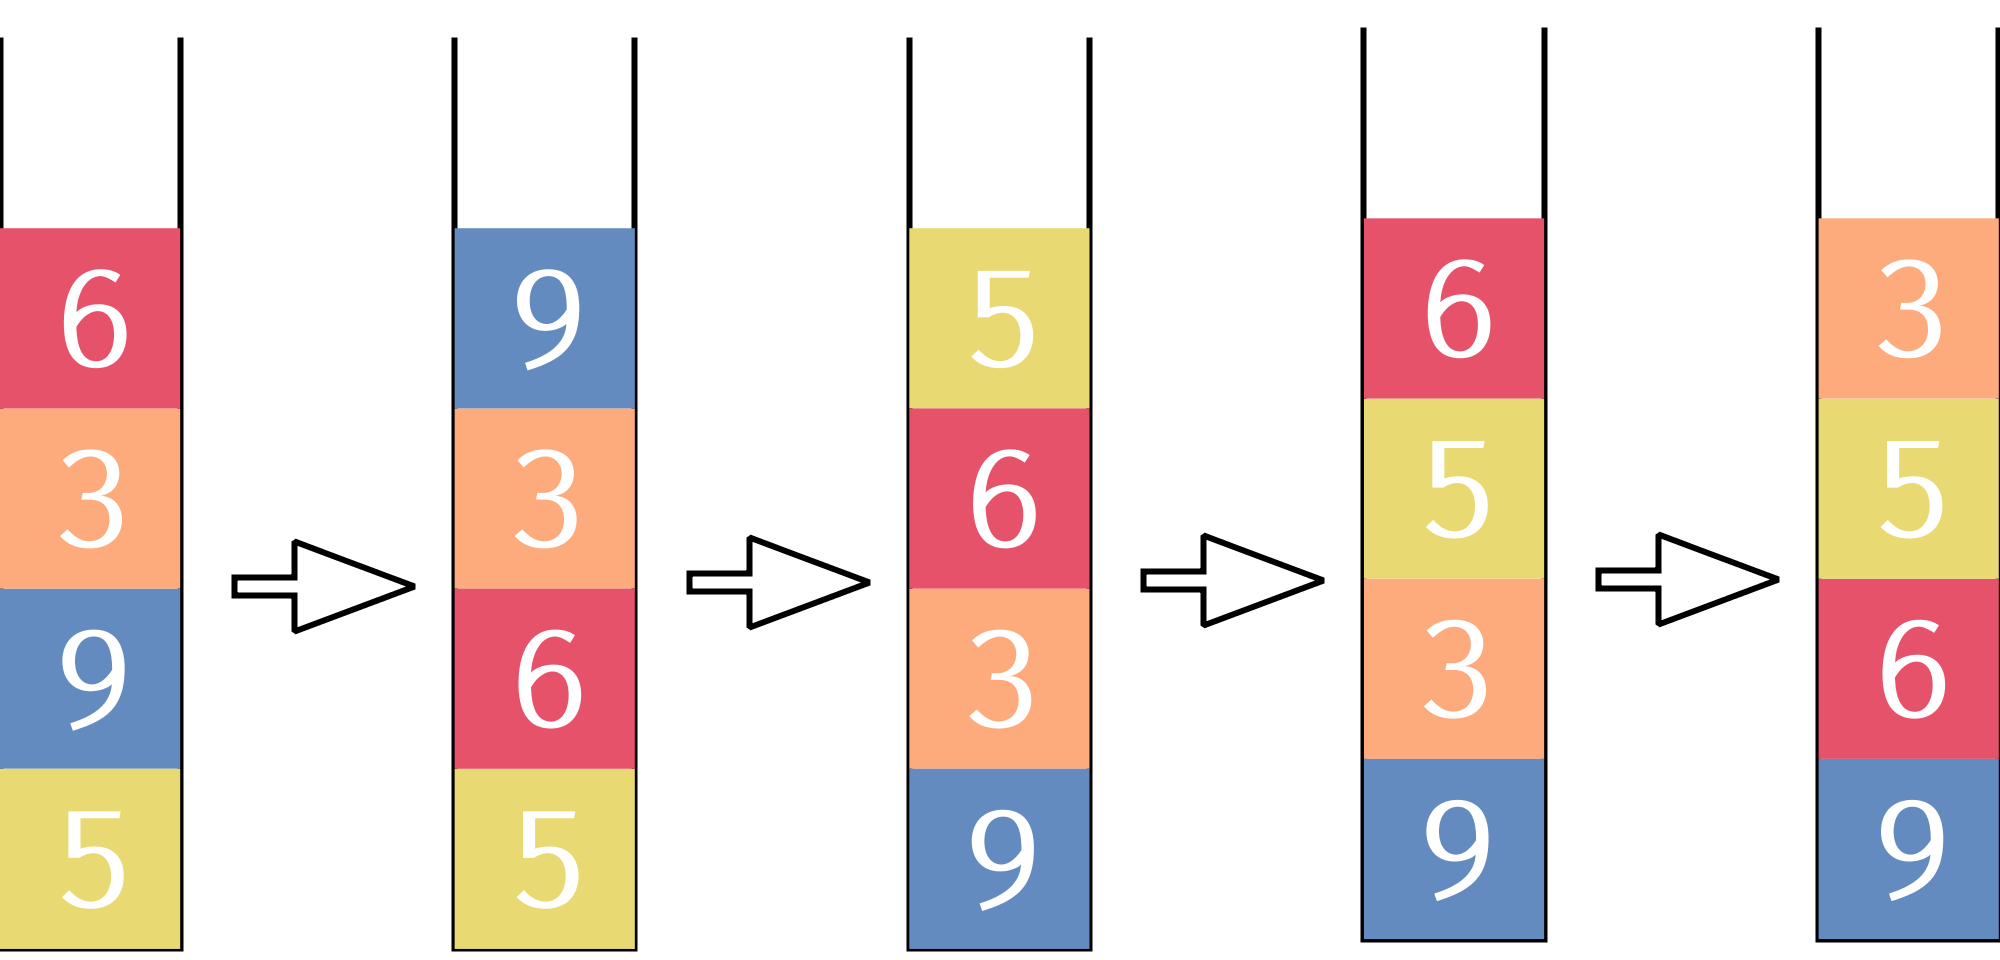
\includegraphics[width=8.1cm]{img/pile3.png}
\end{center}

Créer la fonction \mintinline{python}{tri_crepes} ayant pour paramètre une pile \mintinline{python}{p} . Cette fonction trie la pile \mintinline{python}{p}  selon la
méthode du tri crêpes et ne renvoie rien. On utilisera les fonctions créées dans les questions précédentes.\\

\textbf{Exemple : } Si la pile \mintinline{python}{p} est dans l'état
\begin{center}
      
\includegraphics[width=0.75cm]{img/pile4.png}
\end{center}
alors \mintinline{python}{tri_crepes(p)} la met dans l'état
\begin{center}
      
\includegraphics[width=0.75cm]{img/pile5.png}
\end{center}

\carreauxseyes{16}{8}
\section*{Exercice 1 \small\hfill POO}
\resetquestion

Les participants à un jeu de LaserGame sont répartis en équipes et s'affrontent dans ce jeu de tir, revêtus d'une veste à capteurs et munis d'une arme factice émettant des infrarouges.\\
Les ordinateurs embarqués dans ces vestes utilisent la programmation orientée objet pour modéliser les joueurs. La classe Joueur est définie comme suit :

\begin{pyc}
\begin{minted}{python}
      class Joueur:
            
            def __init__(self, pseudo, identifiant, equipe):
                  self.pseudo = pseudo
                  self.equipe = equipe
                  self.id = identifiant
                  self.nb_de_tirs_emis = 0
                  self.liste_id_tirs_recus = []
                  self.est_actif = True
            
            def tire(self):
                  '''déclenchée par l'appui sur la gachette'''
                  if self.est_actif == True:
                        self.nb_de_tirs_emis = self.nb_de_tirs_emis + 1
            
            def est_determine(self):
                  '''renvoie True si le joueur réalise un
                  grand nombre de tirs'''
                  return self.nb_de_tirs_emis > 500
            
            def subit_un_tir(self, id_recu):
                  '''déclenchée par les capteurs de la veste'''
                  if self.est_actif == True:
                        self.est_actif = False
                        self.liste_id_tirs_recus.append(id_recu)            
\end{minted}
\end{pyc}
\question Parmi les instructions suivantes, entourer celle qui permet de déclarer un objet
\mintinline{python}{joueur1}, instance de la classe \mintinline{python}{Joueur}, correspondant à un joueur dont le pseudo est \mintinline{sql}{Sniper}, dont l'identifiant est \mintinline{sql}{319} et qui est intégré à l'équipe \mintinline{sql}{A}:
\begin{itemize}
      \item \textbf{Instruction 1} :\\ \mintinline{python}{joueur1 = ["Sniper", 319, "A"]}
      \item \textbf{Instruction 2} :\\ \mintinline{python}{joueur1 = new Joueur["Sniper", 319, "A"]}
      \item \textbf{Instruction 3} :\\ \mintinline{python}{joueur1 = Joueur("Sniper", 319, "A")}
      \item \textbf{Instruction 4} :\\ \mintinline{python}{joueur1 = Joueur{"pseudo":"Sniper", "id":319, "equipe":"A"}}
\end{itemize}


\question La méthode \mintinline{python}{subit_un_tir} réalise les actions suivantes :
Lorsqu'un joueur actif subit un tir capté par sa veste, l'identifiant du tireur est
ajouté à l'attribut \mintinline{python}{liste_id_tirs_recus} et l'attribut \mintinline{python}{est_actif} prend la
valeur \mintinline{python}{False} (le joueur est désactivé). Il doit alors revenir à son camp de base pour être de nouveau actif.
\begin{enumalph}
      \item Écrire la méthode \mintinline{python}{redevenir_actif} qui rend à nouveau le joueur actif uniquement s'il était précédemment désactivé.\\

      \carreauxseyes{16}{4}
      \item Écrire la méthode \mintinline{python}{nb_de_tirs_recus} qui renvoie le nombre de tirs reçus par un joueur en utilisant son attribut \mintinline{python}{liste_id_tirs_recus}.\\
      
      \carreauxseyes{16}{4}
\end{enumalph}

\question Lorsque la partie est terminée, les participants rejoignent leur camp de base respectif où un ordinateur, qui utilise la classe \mintinline{python}{Base}, récupère les données.\\
La classe \mintinline{python}{Base} est définie par :
\begin{itemize}
      \item ses attributs :
            \begin{itemize}
                  \item \mintinline{python}{equipe} : nom de l'équipe (str), par exemple, \mintinline{sql}{A} ;
                  \item \mintinline{python}{liste_des_id_de_l_equipe} qui correspond à la liste (list) des identifiants connus des joueurs de l'équipe ;
                  \item \mintinline{python}{score} : score (int) de l'équipe, dont la valeur initiale est 1000.
            \end{itemize}
      \item ses méthodes :
            \begin{itemize}
                  \item \mintinline{python}{est_un_id_allie} qui renvoie \mintinline{python}{True} si l'identifiant passé en paramètre est un identifiant d'un joueur de l'équipe, \mintinline{python}{False} sinon ;
                  \item  \mintinline{python}{incremente_score} qui fait varier l'attribut score du nombre passé en paramètre ;
                  \item  \mintinline{python}{collecte_information} qui récupère les statistiques d'un participant passé en paramètre (instance de la classe \mintinline{python}{Joueur}) pour calculer le score de l'équipe.
            \end{itemize}
\end{itemize}

\begin{pyc}
\begin{minted}{python}
      def collecte_information(self,participant):
            if participant.equipe == self.equipe : # test 1
                  for id in participant.liste_id_tirs_recus:
                        if self.est_un_id_allie(id): # test 2
                              self.incremente_score(-20)
                        else:
                              self.incremente_score(-10)
\end{minted}
\end{pyc}
\begin{enumalph}
      \item Indiquer le numéro du test (test 1 ou test 2) qui permet de vérifier qu'en fin de
      partie un participant égaré n'a pas rejoint par erreur la base adverse.\\

      \carreauxseyes{16}{1.6}

      \item Décrire comment varie quantitativement le score de la base lorsqu'un joueur
      de cette équipe a été touché par le tir d'un coéquipier.

      \carreauxseyes{16}{3.2}
\end{enumalph}

On souhaite accorder à la base un bonus de 40 points pour chaque joueur particulièrement déterminé (qui réalise un grand nombre de tirs).\\

\question Compléter, en utilisant les méthodes des classes \mintinline{python}{Joueur} et \mintinline{python}{Base}, les 2 lignes de codes suivantes qu'il faut ajouter à la fin de la méthode \mintinline{python}{collecte_information} :
\begin{pyc}
      \begin{minted}{python}
            #si le participant réalise un grand nombre de tirs
            ........ 

            #le score de la Base augmente de 40
            .........             
      \end{minted}
\end{pyc}

\end{document}
